\documentclass[tikz,border=5pt]{standalone}
\usepackage[utf8]{inputenc}
\usepackage[T1]{fontenc}
\usepackage{lmodern,amsmath,amssymb}
\usepackage[american]{circuitikz}
\usepackage{pgfplots}
\pgfplotsset{compat=1.18}
\usetikzlibrary{circuits.logic.US,positioning,calc,arrows.meta,patterns,shapes.geometric}
\definecolor{Primary}{HTML}{1F77B4}
\begin{document}
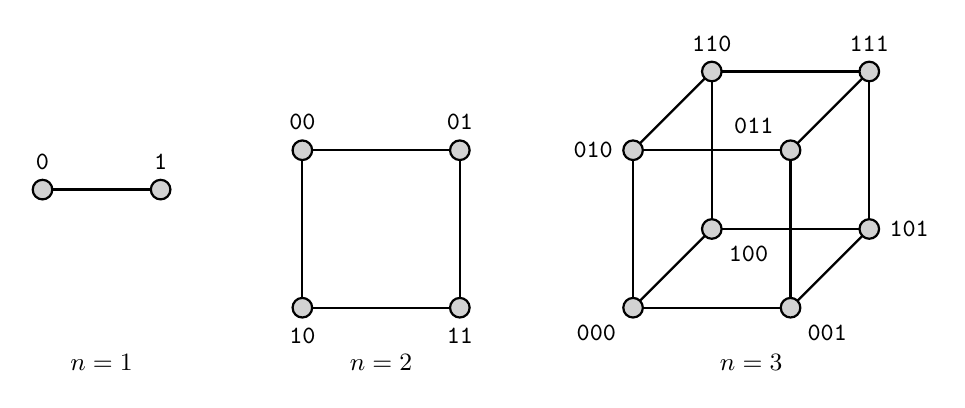
\begin{tikzpicture}[thick,font=\small,
 vertex/.style={circle,draw,fill=gray!35,inner sep=2.5pt},
 every label/.style={font=\small\ttfamily,inner sep=3pt}]
% Ivice su eksplicitne; svaka spaja reci koje se razlikuju u jednom bitu.
\coordinate (a0) at (0,1.5);\coordinate (a1) at (1.5,1.5);
\draw (a0)--(a1);
\node[vertex,label=above:0] at (a0){};
\node[vertex,label=above:1] at (a1){};
\node at (.75,-.7){$n=1$};
\coordinate (b00) at (3.3,2);\coordinate (b01) at (5.3,2);
\coordinate (b10) at (3.3,0);\coordinate (b11) at (5.3,0);
\draw (b00)--(b01) (b01)--(b11) (b11)--(b10) (b10)--(b00);
\foreach \name/\pos/\word in {b00/above/00,b01/above/01,b10/below/10,b11/below/11}
  \node[vertex,label=\pos:\word] at (\name){};
\node at (4.3,-.7){$n=2$};
\coordinate (c000) at (7.5,0);\coordinate (c001) at (9.5,0);
\coordinate (c010) at (7.5,2);\coordinate (c011) at (9.5,2);
\coordinate (c100) at (8.5,1);\coordinate (c101) at (10.5,1);
\coordinate (c110) at (8.5,3);\coordinate (c111) at (10.5,3);
\draw (c000)--(c001) (c001)--(c011) (c011)--(c010) (c010)--(c000);
\draw (c100)--(c101) (c101)--(c111) (c111)--(c110) (c110)--(c100);
\draw (c000)--(c100) (c001)--(c101) (c010)--(c110) (c011)--(c111);
\foreach \name/\pos/\word in {c000/below left/000,c001/below right/001,c010/left/010,c011/above left/011,c100/below right/100,c101/right/101,c110/above/110,c111/above/111}
  \node[vertex,label=\pos:\word] at (\name){};
\node at (9,-.7){$n=3$};
\end{tikzpicture}
\end{document}
